\setcounter{chapter}{0}

\chapter{Tworzenie zbioru danych}
Tworzenie zbioru danych jest bardzo istotnym etapem w uczeniu maszynowym. Od ich jakości oraz formatu zależy skuteczność modelu. Dane użyte do trenowania zostały pobrane ze strony \textit{lichess.org}. Został wykorzystany zbiór \textit{Lichess Elite Database} zawierający rozgrywki graczy na poziomie większym niż 2300, co jest bardzo wysokim wynikiem. Co ważne, zbiór ten nie zawiera powtórzeń, a także rozgrywek czasowych dzięki temu model nie uczy się złych, nietypowych strategii tworzonych pod presją czasu. Pobrany zbiór danych składa się z kilku plików o rozszerzeniu \textit{.pgn}, z których każdy zawiera około miliona partii szachowych

\section{Format danych PGN}
Format PGN jest powszechnie stosowanym sposobem przechowywania partii szachowych. W danym pliku może znajdować się dowolna ilość gier. Każda z nich ma między innymi nazwy graczy, wynik oraz stos ruchów. Taki sposób zapisu jest bardzo efektywny pamięciowo, gdyż nie zapisuje on pozycji na planszy w każdej turze, a jedynie wykonywane ruchy. Dodatkowym atutem jest gotowa biblioteka python-chess do dekodowania pliku oraz rozgrywania partii.

\vspace{0.5cm}

\begin{lstlisting}[
    language=Python, 
    caption=przykład pliku PGN,
    inputencoding=utf8,
    basicstyle=\ttfamily\footnotesize,
    xleftmargin=0.1cm,
    showspaces=false,
    showstringspaces=false,
    showtabs=false,
    keepspaces=true
]
[Event "F/S Return Match"] 
[Site "Belgrade, Serbia JUG"] 
[Date "1992.11.04"] 
[Round "29"] 
[White "Fischer, Robert J."]
[Black "Spassky, Boris V."] 
[Result "1/2-1/2"] 

1. e4 e5 2. Nf3 Nc6 3. Bb5 a6 4. Ba4 Nf6 5. O-O Be7 6. Re1 b5 7. Bb3 d6 ...
\end{lstlisting}
\section{Klasa PGNDataset}
Do przetworzenia danych została stworzona klasa PGNDataset. Jej zadaniem jest utworzenie plików o rozszerzeniu .rdg, które zawierają zserializowany obiekt krotki, która zawiera trzy tablice numpy. Pierwsza z nich przechowuje zakodowane ruchy, druga plansze, a trzecia wyniki partii. Ze względów na dużą ilość danych do przetworzenia, klasa ta działa równolegle, wykorzustując procesy. Każdy proces przetwarza osobny plik \textit{.pgn}, a następnie zapisuje zakodowane dane do osobnego pliku \textit{.rdg}. Dzięki temu czas potrzebny na przetworzenie całego zbioru danych jest znacznie krótszy w przypadku wielordzeniowych procesorów.

\newpage

Każdy plik \textit{.rdg} zawiera trój członową nazwę. Pierwszy człon to id procesu, który go stworzył, drugi to numer porządkowy pliku, a trzeci to ilość zakodowanych gier. Pierwsze człony pełnią role identyfikatora, a trzeci pozwala na stworzenie pasku postępu podczas trenowania modelu.

Ilość zapisanych gier w jednym pliku jest konfigurowalna i można ją ustawić w \textit{config.json} pod kluczem \textit{max\_games\_per\_train\_file}. Dobranie odpowiedniej wartość zależy przedewszystkim od ilości pamięci RAM. Dobrana wartość również może wpłynąć na jakość modelu, gdyż zbyt duża ilość gier może nie umożliwić odpowiedniego wymieszania dużej ilości danych z różnych plików podczas trenowania. 

Dodatkowo klasa ta umożliwia twórzenie zbioru testowego poprzez zapisanie losowych zakodowanych gier do osobnego folderu. Proporcje tego zbioru można również ustawić w pliku konfiguracyjnym pod kluczem \textit{test\_split\_ratio}. W jednym pliku jest zapisywana $test\_split\_ratio * max\_games\_per\_train\_file$ ilość gier.

\section{Kodowanie gier}

Działanie klasy rozpoczyna się od metody \textit{encode directory}, która przyjmuje ścieżke do katalogu z plikami \textit{.pgn}. Następnie iteruje po wszystkich plikach. Dla każdej gry z pliku wywołuje metodę \textit{encode game}, której listing jest przedstawiony pod spodem. Enkoduje ona ruchy, plansze oraz wynik parti i zwraca je w postaci trzech tablic numpy. Po przetworzeniu odpowiedniej ilości gier, są one zapisywane do pliku \textit{.rdg} w postaci krotki. Dodatkowo ze względu na model, który uczy się jedynie ruchów dla białych figur, podczas ruchu czarnych obracana jest plansza po przekątnej wraz z zmianą perspektywy ruchu oraz wyniku parti. Działa to identycznie, tak jakbyśmy w rzeczywistości zamienili się miejscem z przeciwnikiem. Dzięki temu nie trzeba uczyć modelu dwóch różnych strategii dla obu graczy, a jedynie jednej uniwersalnej.

\vspace{0.5cm}

\lstset{style=codeListingStyle}
\begin{lstlisting}[
    language=Python, 
    caption=Metoda encode game,
    inputencoding=utf8
]
def encode_game(self, game: chess.pgn.Game):
        board = BoardPlus()
        moves, boards, wins = [], [], []

        for move in game.mainline_moves():
            real_board.push(move)
            if board.changed_perspective:
                move = BoardPlus.change_move_perspective(move)

            moves.append(board.encode_move(move))
            boards.append(board.encode())
            wins.append(self.white_win(game) * (1 if not board.changed_perspective else -1))
            board.better_push(move)

            board.change_perspective()
        return np.array(moves), np.array(boards), np.array(wins)
\end{lstlisting}

\vspace{1cm}

\section{Przechowywanie zakodowanych gier w pamięci programu}
Dane w postaci list zwracane przez metodę \textit{encode game} są dodawane do kolejnych trzech list: \textit{games move}, \textit{games board} oraz \textit{games win}. Po przetworzeniu odpowiedniej ilości gier są one scalane za pomocą metody \textit{concatenate} i zapisywane do pliku. Taki nietypowy sposób przechowywania został zastosowany ze względów wydajnościowych. Przy użyciu jednowymiarowych list, po każdym wywołaniu metody \textit{enocde game}, trzeba by używać \textit{concatenate} do scalania danych, co jest bardzo nieefektywne. Wraz z wielkością list, a więc kolejną iteracją, czas wykonania rośnie co można zaobserwować na rysunku \ref{fig:concatenate_time}. Zastosowanie list dwuwymiarowych pozwala na uniknięcie tego problemu, gdyż metoda \textit{concatenate} jest wywoływana tylko raz. Dodatkowo przed zapisem do plików dane z list są mieszane w losowej kolejności, aby poprawić jakość trenowania modelu.

\hspace{0.5cm}

\lstset{style=codeListingStyle}
\begin{lstlisting}[
    language=Python, 
    caption=Fragment metody encode directory,
    inputencoding=utf8
]
game_moves, game_boards, game_wins = self.encode_game(game)

if len(game_moves) == 0 or len(game_boards) == 0 or len(game_wins) == 0:
    continue
games_move.append(game_moves)
games_board.append(game_boards)
games_win.append(game_wins)

PGNDataset.number_converted_games += 1
if PGNDataset.number_converted_games % max_games_in_file == 0:
    moves, boards, wins = np.concatenate(games_move), np.concatenate(games_board), np.concatenate(games_win)
    PGNDataset.save_games_data_to_file((moves, boards, wins), output_path)
    games_move, games_board, games_win = [], [], []
\end{lstlisting}

\vspace{1cm}

\begin{figure}[h!]
    \centering
    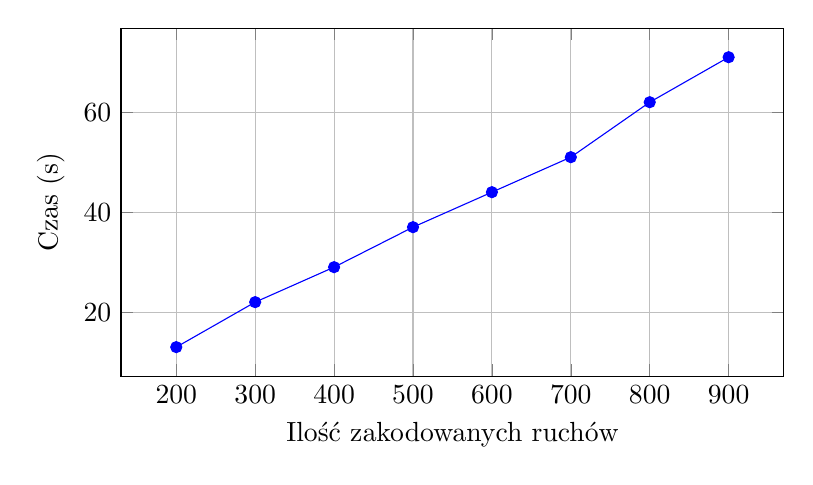
\begin{tikzpicture}
    \begin{axis}[
        xlabel={Ilość zakodowanych ruchów},
        ylabel={Czas (s)},
        grid=major,
        legend pos=north east,
        width=10cm,
        height=6cm
    ]
    \addplot[blue, mark=*] coordinates {
        (200, 13)
        (300, 22)
        (400, 29)
        (500, 37)
        (600, 44)
        (700, 51)
        (800, 62)
        (900, 71)
    };
    \end{axis}
    \end{tikzpicture}
    \caption{Czas wykonania metod concatenate po każdym zakodowaniu gry}
    \label{fig:concatenate_time}
\end{figure}

